\documentclass[letter,12pt]{article}
\usepackage[paperheight=27.94cm,paperwidth=21.59cm,bindingoffset=0in,left=3cm,right=2.0cm, top=3.5cm,bottom=2.5cm, headheight=200pt, headsep=1.0\baselineskip]{geometry}
\usepackage{graphicx,lastpage}
\usepackage{upgreek}
\usepackage{censor}
\usepackage[spanish,es-tabla]{babel}
\usepackage{pdfpages}
\usepackage{tabularx}
\usepackage{graphicx}
\usepackage{adjustbox}
\usepackage{xcolor}
\usepackage{colortbl}
\usepackage{rotating}
\usepackage{multirow}
\usepackage[utf8]{inputenc}
\usepackage{float}
\usepackage[hidelinks]{hyperref}
\usepackage{listings}
\usepackage{listingsutf8}
\usepackage{needspace}

\lstset{
    inputencoding=utf8/latin1,
    basicstyle=\ttfamily\scriptsize,
    breaklines=true,
    frame=single,
    numbers=left,
    numberstyle=\tiny,
    showstringspaces=false,
    columns=fullflexible,
    keepspaces=true,
    literate={í}{{\'i}}1
}

\renewcommand{\tablename}{Tabla}
\usepackage{fancyhdr}
\pagestyle{fancy}


%
\begin{document}
%
   \title{\Huge{Informe Laboratorio 4}}

   \author{\textbf{Sección 3} \\  \\Edicson Solar Salinas \\ e-mail: edicson.solar@mail.udp.cl}
          
   \date{26 de Octubre a 1 de Noviembre de 2026}

   \maketitle
   
   \begingroup
   \small
   \tableofcontents
   \endgroup
 
  \newpage
  

\section{Descripción}
Usted trabaja en una empresa especializada en la transferencia segura de información, archivos y contenido digital. Antes de incorporarse al desarrollo y operación de los sistemas reales de la organización, se le solicita realizar una demostración técnica que permita evaluar sus conocimientos en redes, protocolos de comunicación y criptografía.

Para ello, deberá implementar y configurar un servidor SSH, definiendo los mecanismos criptográficos utilizados para proteger la comunicación. Posteriormente, deberá establecer una conexión con el servidor y capturar el tráfico de red utilizando Wireshark.

A partir del análisis de los paquetes capturados, deberá identificar qué información puede ser observada por un tercero que tuviera acceso al tráfico de red y determinar qué elementos de la comunicación están protegidos mediante cifrado y cuáles pueden ser visibles, con el objetivo de evaluar el nivel de seguridad proporcionado por el protocolo SSH.

Finalmente, se le proporcionará una captura de tráfico de red obtenida mediante Wireshark. En ella se encuentran diversos mensajes correspondientes a transacciones que han sido cifrados mediante RSA.

El objetivo de esta actividad es analizar la captura de tráfico, identificar los paquetes que contienen la información cifrada y desarrollar un programa en Python que permita recuperar el contenido original.

\section{Actividades}
\subsection{Configuración y análisis de SSH}
\subsubsection{Implementación y configuración del servidor SSH}

    Generar un contenedor Docker que permita ejecutar un servidor SSH accesible desde el equipo cliente (su computador). Posteriormente, configure el servidor mediante un archivo \texttt{sshd\_config}, en el cual deberá especificar los algoritmos criptográficos utilizados durante la comunicación SSH: \texttt{curve25519-sha256}, \texttt{aes256-ctr}, \texttt{hmac-sha2-256} y \texttt{ssh-ed25519}. Por último, documente la función que cumple cada algoritmo dentro del proceso de establecimiento y comunicación de una conexión SSH.


\subsubsection{Análisis de paquetes SSH en Wireshark}

    Una vez completada la configuración del servidor SSH, deberá analizar el tráfico de red generado durante el establecimiento de la conexión utilizando Wireshark.

    Para ello, antes de realizar la conexión SSH, inicie la captura de tráfico en la interfaz de red correspondiente. Posteriormente, establezca una conexión con el servidor utilizando su máquina como cliente y analice los paquetes intercambiados durante el proceso de conexión.

    A partir del análisis realizado, responda la siguiente pregunta:

    ¿Qué información es posible identificar a partir de los paquetes capturados? Mencione y explique al menos tres elementos que puedan observarse en el tráfico de la conexión SSH.

  %  \item Adicionalmente, se indica que es posible configurar el servidor SSH para utilizar RSA como algoritmo de clave de host. Para comprobar si se han generado las claves RSA, puede ejecutar el siguiente comando dentro del servidor:
    
  %  "ls -l /etc/ssh/ssh\_host\_rsa\_key*"
    
   % Si existen dos archivos, uno correspondiente a la clave privada (`ssh\_host\_rsa\_key`) y otro a la clave pública (`ssh\_host\_rsa\_key.pub`), significa que ambas claves están presentes. Tenga presente que su existencia no garantiza que el servidor esté configurado para utilizarlas. 


\subsection{Análisis de captura de tráfico antigua}

\subsubsection{Análisis de los mecanismos criptográficos}
Se le solicita analizar una captura de tráfico de red antigua, en formato .pcap, que contiene transacciones financieras cifradas mediante una combinación de criptografía asimétrica y simétrica. Para realizar la actividad, se le proporcionarán la captura y las claves pública y privada RSA correspondientes. Deberá identificar los paquetes relevantes y analizar el mecanismo de cifrado utilizado, considerando que RSA se emplea para cifrar un PIN de cuatro dígitos mediante OAEP con SHA-256, mientras que AES-GCM se utiliza para proteger el contenido de las transacciones financieras.

\subsubsection{Recuperación del PIN y derivación de la clave AES}
El primer paquete relevante de la captura contiene la etiqueta RSA\_PIN, seguida de una salt de 16 bytes y del PIN cifrado mediante RSA. Deberá identificar y extraer estos campos, utilizar la clave privada RSA proporcionada para recuperar el PIN y, posteriormente, derivar la clave AES de 256 bits mediante Scrypt. Para ello, deberá utilizar el PIN recuperado, la salt extraída de la captura y los siguientes parámetros: (n=2**{14}), (r=8) y (p=1). Explique la función de la salt y por qué es necesario utilizar los mismos parámetros para obtener la clave AES original.

\subsubsection{Descifrado de las transacciones y análisis final}
Una vez obtenida la clave AES, deberá identificar todos los paquetes que contienen transacciones cifradas mediante AES-GCM. Para cada paquete, deberá extraer el nonce de 12 bytes y utilizarlo junto con la clave derivada y el texto cifrado para recuperar los mensajes originales, verificando su autenticidad. Implemente el procedimiento completo en un script de Python y presente las transacciones recuperadas en su formato original, incluyendo el identificador, el remitente, el destinatario y el monto. Documente el procedimiento realizado e incluya evidencias de los resultados obtenidos.
\begin{figure}[H]
    \centering
    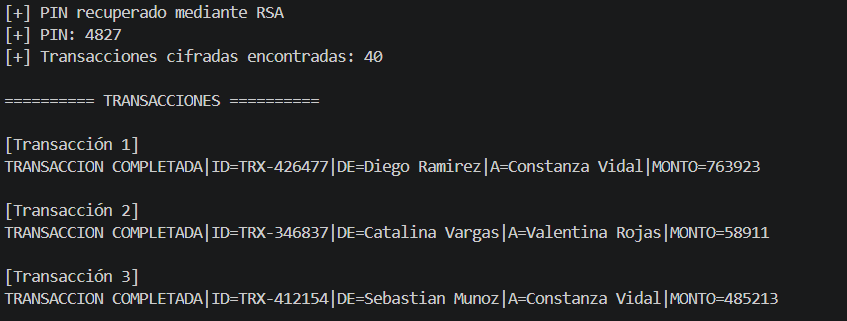
\includegraphics[width=0.9\linewidth]{../evidencias/capturas_informe/Screenshot 2026-10-15 164449.png}
    \caption{Ejemplo del resultado}
    \label{fig:placeholder}
\end{figure}

Finalmente, responda la siguiente pregunta, justificando su respuesta: ¿Sería posible descifrar los mensajes capturados utilizando las claves pública y privada RSA en cifrados PQC (Criptografía post-cuántica)?

\section{Desarrollo de actividades}

\subsection{Actividad 1}
    \subsubsection{Dockerfile}

    Usé una imagen base \texttt{debian:bookworm-slim} e instalé
    \texttt{openssh-server}. Dentro de la imagen creé el usuario \texttt{lab4}, copié su
    clave pública y la configuración del servidor, y generé una clave de host Ed25519. La
    autenticación del usuario quedó limitada a clave pública.

    Antes de terminar la construcción ejecuté \texttt{sshd -t}. De esta forma, una
    configuración inválida hace fallar el build en vez de aparecer recién al iniciar el
    contenedor. El proceso principal se ejecuta en primer plano con \texttt{sshd -D -e}.

    \begin{figure}[H]
        \centering
        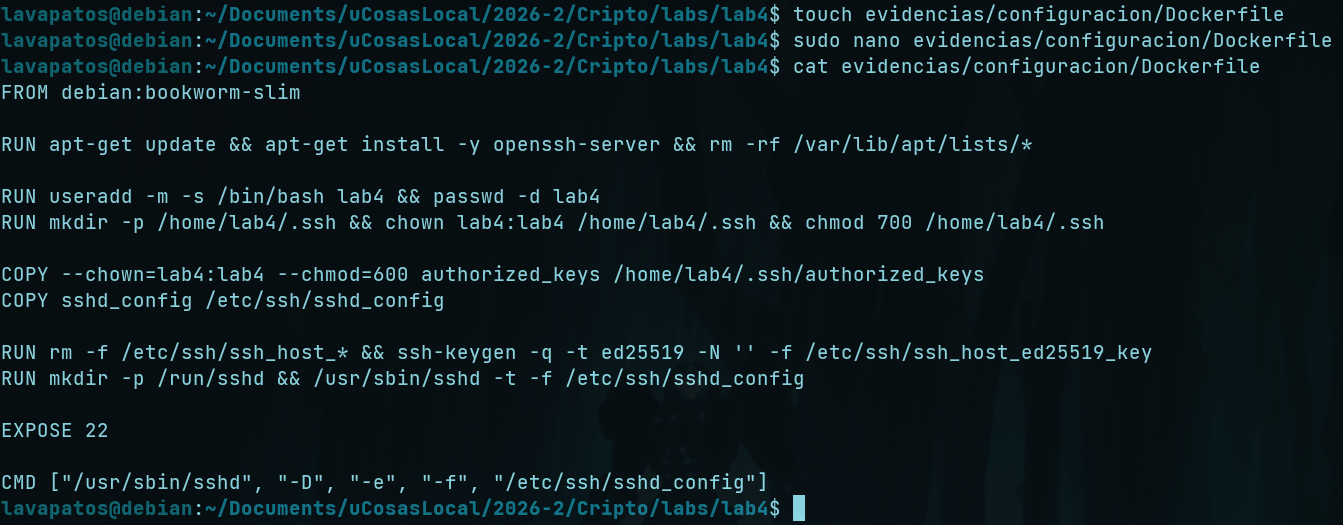
\includegraphics[width=0.95\linewidth]{../evidencias/capturas_informe/01_dockerfile.png}
        \caption{Dockerfile utilizado para construir el servidor SSH.}
        \label{fig:dockerfile}
    \end{figure}

    Construí la imagen con el nombre \texttt{lab4-ssh:2026}. El proceso terminó
    correctamente y creó la imagen local, como se observa en la Figura
    \ref{fig:docker-build}.

    \begin{figure}[!htbp]
        \centering
        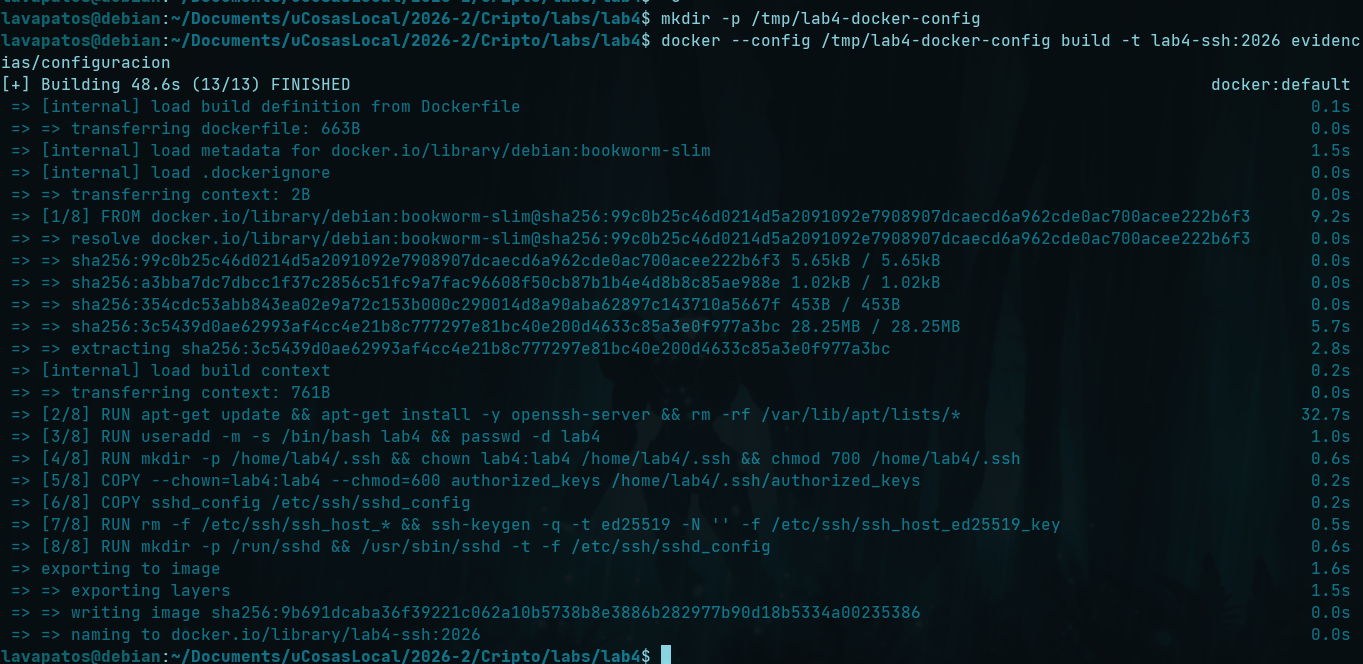
\includegraphics[width=0.90\linewidth]{../evidencias/capturas_informe/02_docker_build.png}
        \caption{Construcción correcta de la imagen \texttt{lab4-ssh:2026}.}
        \label{fig:docker-build}
    \end{figure}

    Después inicié el contenedor \texttt{lab4-ssh-server}. El puerto 22 del contenedor se
    publicó solamente como \texttt{127.0.0.1:22222}, por lo que el servidor quedó accesible
    desde el mismo equipo y no desde otras interfaces de red.

    \begin{figure}[!htbp]
        \centering
        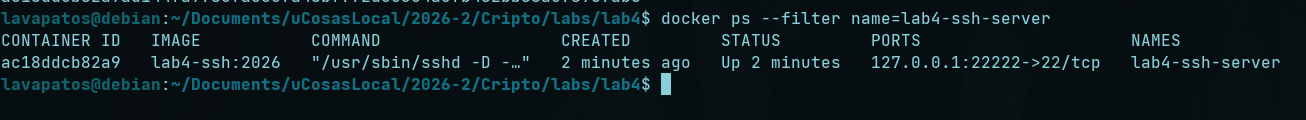
\includegraphics[width=0.95\linewidth]{../evidencias/capturas_informe/04_contenedor_activo.png}
        \caption{Contenedor activo y puerto SSH publicado únicamente en loopback.}
        \label{fig:contenedor-activo}
    \end{figure}

    El registro del contenedor confirmó que \texttt{sshd} quedó escuchando en el puerto 22.
    Dentro del contenedor aparece \texttt{0.0.0.0}, pero la publicación de Docker en el
    equipo anfitrión continúa limitada a \texttt{127.0.0.1:22222}.

    \begin{figure}[!htbp]
        \centering
        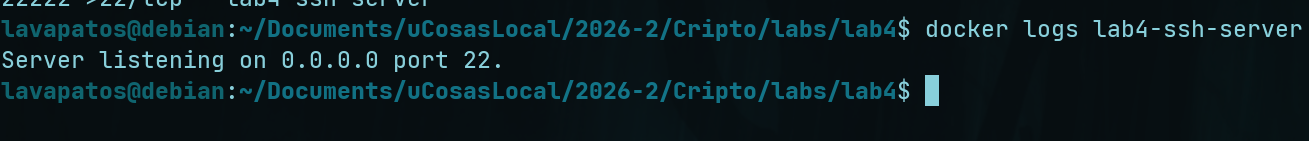
\includegraphics[width=0.95\linewidth]{../evidencias/capturas_informe/05_sshd_escuchando.png}
        \caption{Servidor SSH escuchando correctamente dentro del contenedor.}
        \label{fig:sshd-escuchando}
    \end{figure}

    \subsubsection{Configuración del servidor}

    En \texttt{sshd\_config} fijé de forma explícita los cuatro algoritmos pedidos. La
    configuración usa \texttt{curve25519-sha256} para el intercambio de claves,
    \texttt{aes256-ctr} para el cifrado, \texttt{hmac-sha2-256} para la integridad y
    \texttt{ssh-ed25519} como algoritmo de clave de host.

    También deshabilité el inicio de sesión por contraseña y permití solamente
    autenticación por clave pública para el usuario \texttt{lab4}. El acceso de
    \texttt{root} y los reenvíos de X11, agente, puertos y túneles quedaron desactivados.
    La configuración completa utilizada se muestra en la Figura
    \ref{fig:sshd-config}.

    \begin{figure}[H]
        \centering
        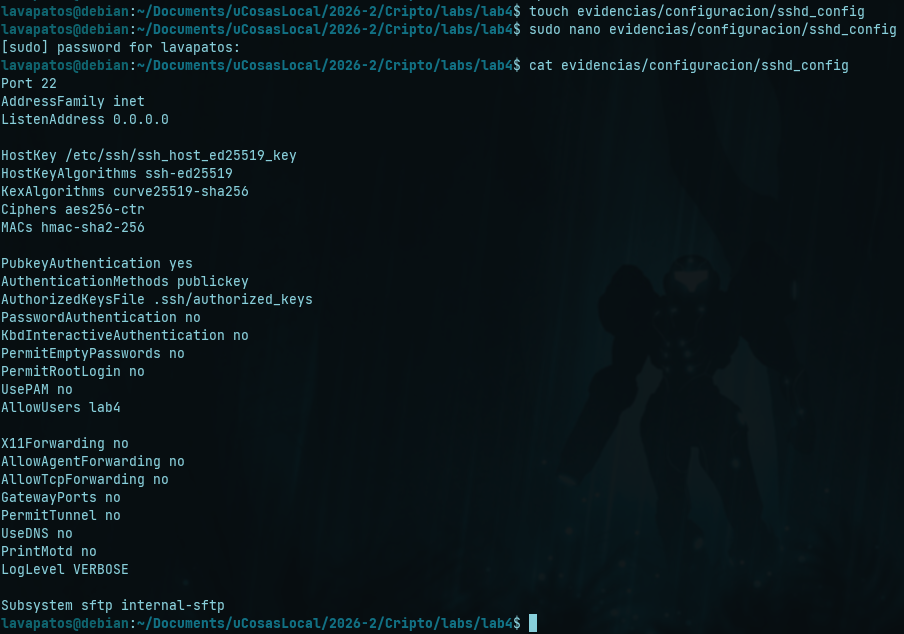
\includegraphics[width=0.82\linewidth]{../evidencias/capturas_informe/04_sshd_config_algoritmosV2.png}
        \caption{Configuración aplicada al servidor SSH.}
        \label{fig:sshd-config}
    \end{figure}

    Para comprobar que el servidor cargó el archivo y no solamente que este contenía los
    valores correctos, consulté su configuración efectiva con \texttt{sshd -T}. La salida
    confirmó exactamente \texttt{curve25519-sha256}, \texttt{aes256-ctr},
    \texttt{hmac-sha2-256} y \texttt{ssh-ed25519}.

    \begin{figure}[H]
        \centering
        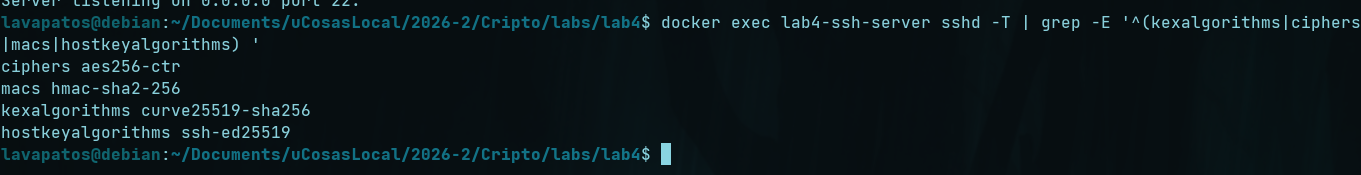
\includegraphics[width=0.95\linewidth]{../evidencias/capturas_informe/06_algoritmos_efectivos.png}
        \caption{Algoritmos efectivos informados por \texttt{sshd -T}.}
        \label{fig:algoritmos-efectivos}
    \end{figure}

    \Needspace{10\baselineskip}
    \subsubsection{Explicación de los algoritmos utilizados}

    Los algoritmos cumplen tareas distintas dentro de SSH. No son cuatro alternativas para
    hacer lo mismo, sino que se usan juntos durante el establecimiento y la comunicación de
    la sesión.

    \paragraph{\texttt{curve25519-sha256}.}
    Lo usé para el intercambio de claves. El cliente y el servidor usan X25519 para calcular
    un secreto compartido sin enviarlo directamente por la red. SHA-256 se usa en el hash
    del intercambio, que después participa en la generación de las claves de sesión. Este
    algoritmo no cifra por sí solo el tráfico y tampoco autentica al servidor. Su uso en
    SSH está definido en la sección 3 de la \href{https://www.rfc-editor.org/rfc/rfc8731.html#section-3}{RFC 8731}.

    \paragraph{\texttt{aes256-ctr}.}
    Es el algoritmo que cifra el tráfico SSH después del intercambio de claves. Usa AES con
    una clave de 256 bits y trabaja en modo contador. Su función es dar confidencialidad al
    contenido de los paquetes. No comprueba si un paquete fue modificado, porque esa tarea
    corresponde al HMAC. Los modos AES en contador para SSH están definidos en la sección 4
    de la \href{https://www.rfc-editor.org/rfc/rfc4344.html#section-4}{RFC 4344}.

    \paragraph{\texttt{hmac-sha2-256}.}
    Comprueba la integridad de cada paquete mediante HMAC con SHA-256. El cálculo incluye el
    número de secuencia y el paquete SSH sin cifrar. Si alguien cambia el contenido durante
    el envío, la verificación ya no coincide y el receptor puede detectar la alteración. Este
    algoritmo no cifra el tráfico. \texttt{hmac-sha2-256} está especificado en la sección 2
    de la \href{https://www.rfc-editor.org/rfc/rfc6668.html#section-2}{RFC 6668}, sobre el
    mecanismo de integridad descrito por la \href{https://www.rfc-editor.org/rfc/rfc4253.html#section-6.4}{RFC 4253}.

    \paragraph{\texttt{ssh-ed25519}.}
    Lo usé como algoritmo de firma para autenticar al servidor. El servidor firma el hash
    del intercambio con su clave privada Ed25519 y el cliente verifica la firma con la clave
    pública. Así se comprueba que el servidor posee la clave privada asociada a la huella
    presentada durante la conexión. Ed25519 firma, pero no cifra. En este laboratorio también
    usé una clave Ed25519 para autenticar al usuario \texttt{lab4}. Su uso como algoritmo de
    clave pública de SSH está definido en la \href{https://www.rfc-editor.org/rfc/rfc8709.html}{RFC 8709}.

    En conjunto, Curve25519 establece el secreto compartido, Ed25519 autentica el
    intercambio, AES-256-CTR cifra los paquetes y HMAC-SHA-256 comprueba su integridad.

    \subsubsection{Conexión cliente-servidor}

    Me conecté desde el equipo anfitrión al servidor publicado en
    \texttt{127.0.0.1:22222}. Para autenticar al usuario utilicé la clave privada Ed25519
    creada exclusivamente para este laboratorio. En la primera conexión el cliente mostró
    la huella de la clave de host Ed25519 y la acepté para guardarla en
    \texttt{known\_hosts}.

    La conexión no solicitó contraseña y abrió el prompt
    \texttt{lab4@ac18ddcb82a9}. Finalmente ejecuté \texttt{whoami} dentro del servidor y la
    respuesta fue \texttt{lab4}, lo que confirma que la sesión se estableció dentro del
    contenedor con el usuario esperado.

    \begin{figure}[H]
        \centering
        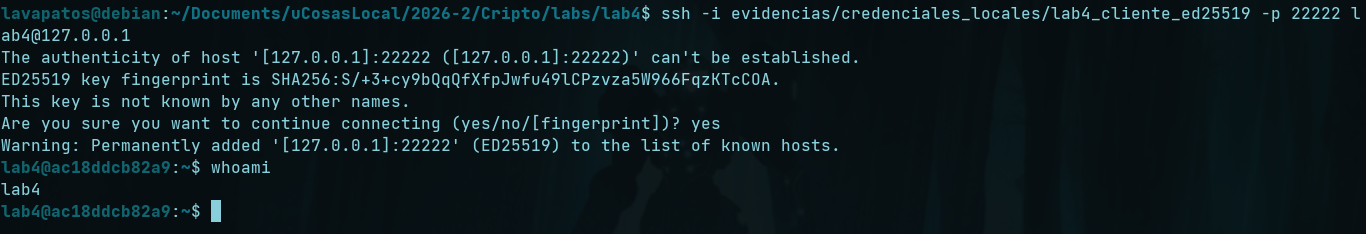
\includegraphics[width=0.98\linewidth]{../evidencias/capturas_informe/07_conexion_ssh_funcional.png}
        \caption{Conexión SSH funcional y comprobación del usuario remoto.}
        \label{fig:conexion-ssh}
    \end{figure}

    \subsubsection{Análisis de tráfico}

    Capturé la conexión sobre la interfaz \texttt{lo} usando el filtro
    \texttt{tcp port 22222}. La captura guardada contiene 38 paquetes. Aunque el contenido
    de la sesión queda cifrado después del intercambio de claves, antes de ese punto todavía
    es posible observar información necesaria para establecer la conexión.

    \noindent\textbf{1. Establecimiento de la conexión TCP.}\par
    Las tramas 1, 2 y 3 muestran el intercambio \texttt{SYN}, \texttt{SYN, ACK} y
    \texttt{ACK}. También se observan el puerto efímero \texttt{52804} del cliente y el
    puerto \texttt{22222} del servidor. Ambas direcciones IP son \texttt{127.0.0.1} porque
    la prueba se realizó completamente sobre loopback. Estos datos permiten reconocer los
    extremos y confirmar que la conexión TCP se estableció correctamente.

    \begin{figure}[H]
        \centering
        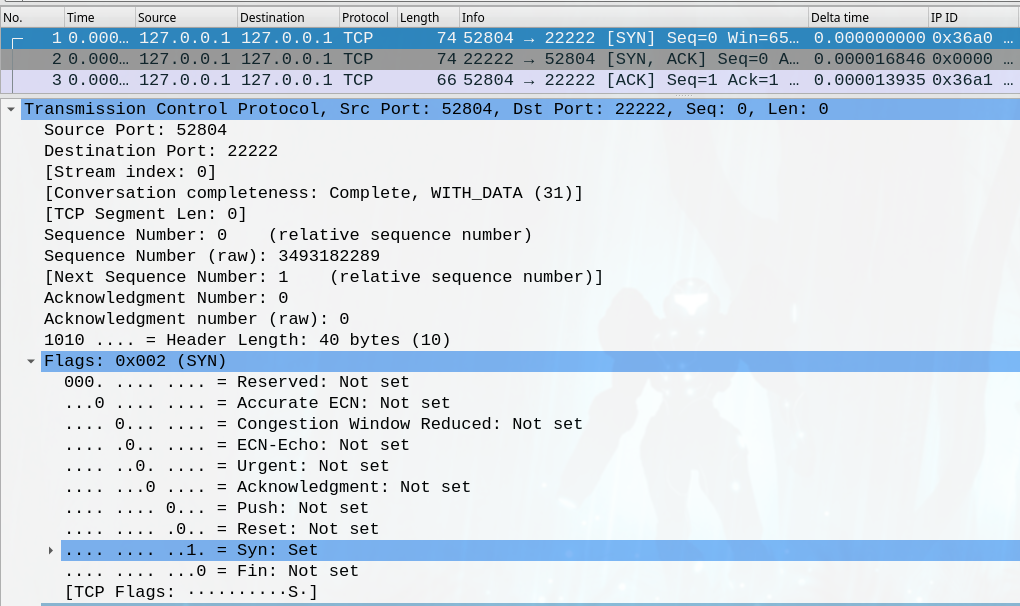
\includegraphics[width=0.95\linewidth]{../evidencias/capturas_informe/09_wireshark_tcp_syn.png}
        \caption{Handshake TCP de tres pasos antes de iniciar SSH.}
        \label{fig:wireshark-tcp}
    \end{figure}

    \Needspace{8\baselineskip}
    \noindent\textbf{2. Versiones del protocolo SSH.}\par
    Antes de activar el cifrado, cliente y servidor intercambian su cadena de identificación.
    En la trama 4 se observa \texttt{SSH-2.0-OpenSSH\_9.2p1 Debian-2+deb12u10} y la dirección
    \texttt{client-to-server}. Esta información revela la versión del protocolo y la
    implementación utilizada, pero no contiene la clave privada ni las credenciales del
    usuario.

    \begin{figure}[H]
        \centering
        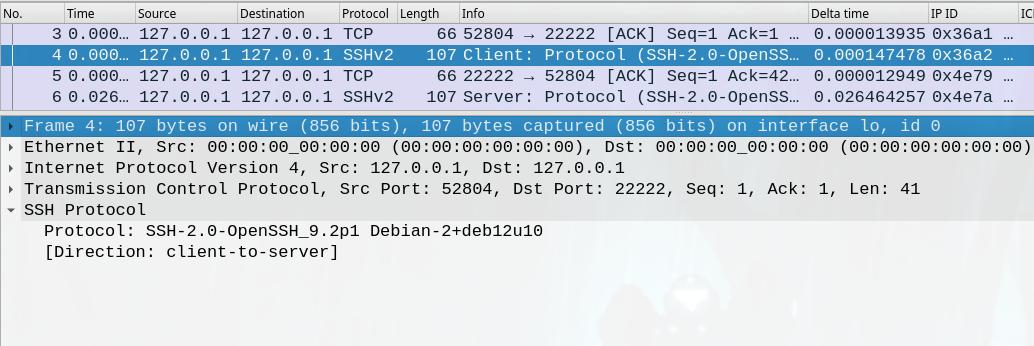
\includegraphics[width=0.95\linewidth]{../evidencias/capturas_informe/10_wireshark_version_ssh.png}
        \caption{Cadena de versión SSH enviada antes de activar el cifrado.}
        \label{fig:wireshark-version}
    \end{figure}

    \noindent\textbf{3. Algoritmos ofrecidos en KEXINIT.}\par
    La trama 9 corresponde al mensaje KEXINIT del servidor. En ella aparecen las cuatro
    propuestas configuradas:
    \begin{itemize}
        \item Intercambio de claves: \texttt{curve25519-sha256}.
        \item Clave de host: \texttt{ssh-ed25519}.
        \item Cifrado: \texttt{aes256-ctr}.
        \item Integridad: \texttt{hmac-sha2-256}.
    \end{itemize}
    AES y HMAC se anuncian por separado para las direcciones cliente-servidor y
    servidor-cliente. También aparece una extensión de negociación estricta de OpenSSH:
    \begin{center}
        \texttt{kex-strict-s-v00@openssh.com}
    \end{center}
    Esta extensión no es un segundo algoritmo KEX configurado por mí.

    \begin{figure}[!htbp]
        \centering
        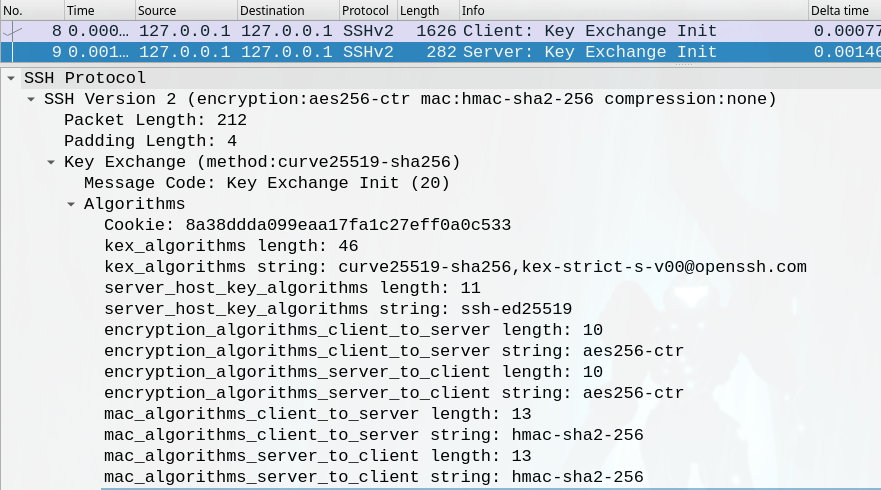
\includegraphics[width=0.95\linewidth]{../evidencias/capturas_informe/11_wireshark_kex_algoritmos_servidor.png}
        \caption{KEXINIT del servidor con los cuatro algoritmos configurados.}
        \label{fig:wireshark-kexinit}
    \end{figure}

    Por lo tanto, un observador puede conocer direcciones, puertos, tiempos, tamaños,
    versiones y algoritmos negociados. Después del mensaje \texttt{New Keys}, los comandos,
    las credenciales y el contenido transportado por la sesión ya no aparecen en texto plano.

\subsection{Actividad 2}
    \subsubsection{Identificación del paquete RSA\_PIN}

    La captura oficial contiene 41 paquetes TCP enviados desde
    \texttt{10.10.10.10:49152} hacia \texttt{10.10.10.20:4444}. Para localizar el paquete
    que transporta el PIN usé el filtro de Wireshark
    \verb|tcp.payload contains "RSA_PIN"|.

    El filtro encontró solamente la trama 1. Su payload tiene 280 bytes y comienza con la
    etiqueta ASCII \texttt{RSA\_PIN|}. Después de los 8 bytes de la etiqueta aparecen los
    16 bytes de salt y los 256 bytes del ciphertext RSA. En esta etapa se identifica la
    estructura, pero el PIN todavía no es visible en texto plano.

    \begin{figure}[H]
        \centering
        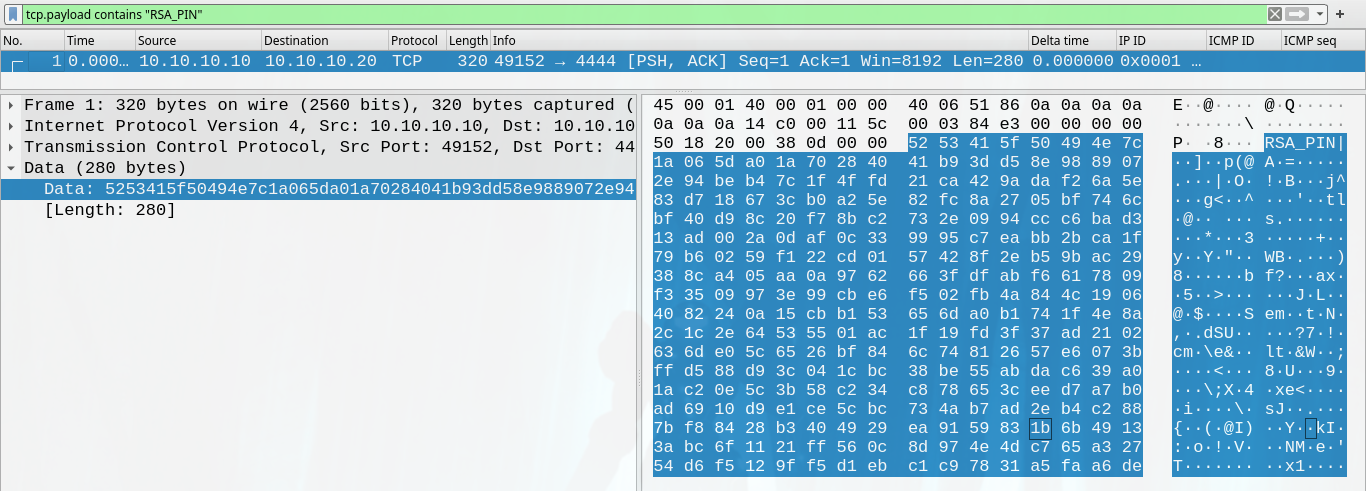
\includegraphics[width=0.98\linewidth]{../evidencias/capturas_informe/12_wireshark_rsa_pin.png}
        \caption{Trama 1 identificada mediante la etiqueta \texttt{RSA\_PIN|}.}
        \label{fig:rsa-pin}
    \end{figure}

    \subsubsection{Identificación de los paquetes AESGCM}

    Para separar las transacciones usé el filtro
    \verb|tcp.payload contains "AESGCM"|. Wireshark mostró 40 coincidencias, que
    corresponden a las tramas 2 a 41. Todas comienzan con la etiqueta ASCII
    \texttt{AESGCM|}.

    Cada payload contiene, después de la etiqueta, un nonce de 12 bytes, el ciphertext de
    largo variable y un tag de autenticación de 16 bytes. La Figura
    \ref{fig:aesgcm-paquetes} muestra el primer paquete seleccionado y el contador
    \texttt{Displayed: 40} en la barra inferior.

    \begin{figure}[H]
        \centering
        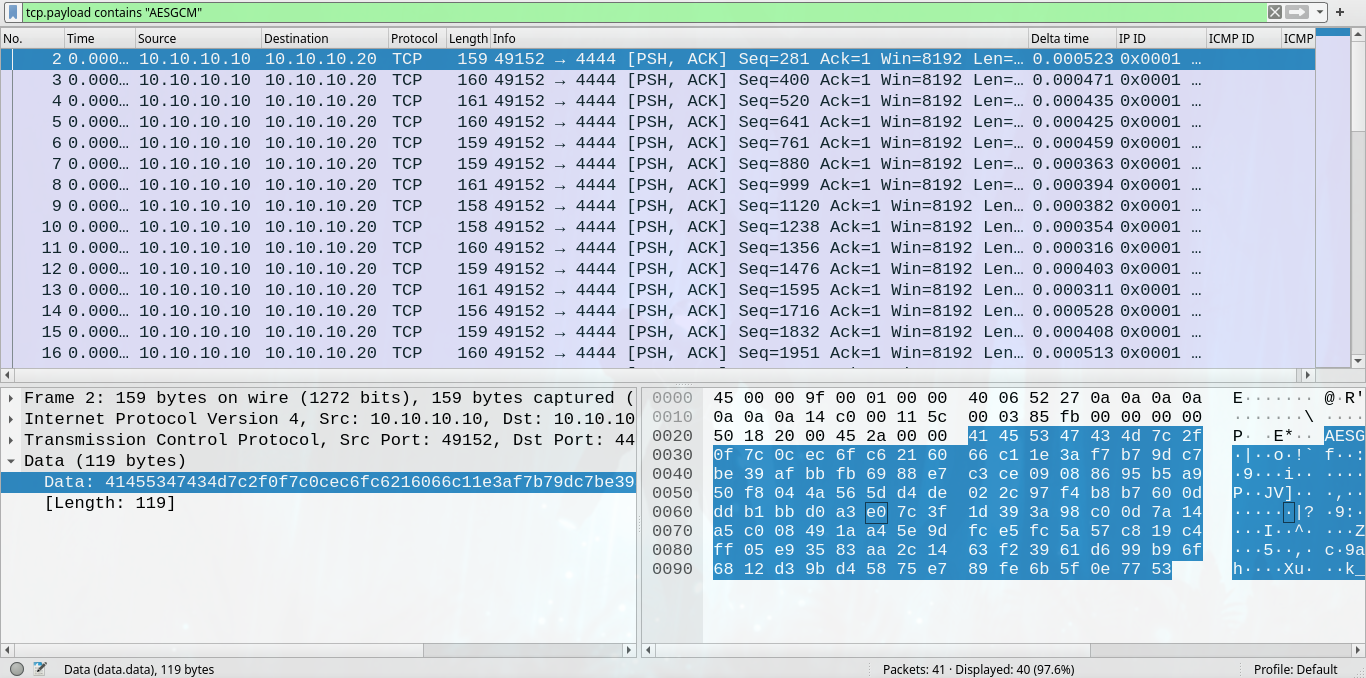
\includegraphics[width=0.98\linewidth]{../evidencias/capturas_informe/13_wireshark_aesgcm.png}
        \caption{Cuarenta paquetes identificados mediante la etiqueta \texttt{AESGCM|}.}
        \label{fig:aesgcm-paquetes}
    \end{figure}

    \subsubsection{Recuperación del PIN y derivación de la clave AES}

    Leí el payload TCP de la trama 1 y separé sus campos usando posiciones fijas. Los
    primeros 8 bytes corresponden a \texttt{RSA\_PIN|}; los bytes 8 a 23 contienen la salt
    de 16 bytes y, desde el byte 24 hasta el final, se encuentra el ciphertext RSA de 256
    bytes.

    La salt extraída fue:
    \begin{center}
        \texttt{1a065da01a70284041b93dd58e988907}
    \end{center}
    El ciphertext comienza con
    \texttt{2e94beb47c1f4ffd21ca429adaf26a5e}. Lo descifré con la clave privada RSA
    entregada, usando OAEP con SHA-256 y MGF1-SHA-256. El resultado fue el PIN
    \texttt{4827}.

    La salt no es una clave secreta. Su función es hacer que la derivación produzca un
    resultado distinto aunque se repita el mismo PIN y dificultar el uso de tablas
    precalculadas. En este caso es especialmente importante porque un PIN de cuatro dígitos
    tiene pocas combinaciones posibles.

    Con el PIN recuperado como entrada y la salt anterior derivé 32 bytes mediante Scrypt.
    Usé exactamente $n=2^{14}$, $r=8$ y $p=1$. El parámetro $n$ determina el costo de
    cómputo y memoria de la derivación, $r$ controla el tamaño de los bloques internos y
    $p$ indica el grado de paralelización. Scrypt es determinista, por lo que cambiar la
    salt o cualquiera de esos valores produciría otra clave y el descifrado AES-GCM
    fallaría.

    La clave AES-256 obtenida fue:
    \begin{center}
        \texttt{f64d739ad8bd559fcd4bde7b9aecb83ff28d200331da635d7409b7133b16eab7}
    \end{center}

    \begin{figure}[H]
        \centering
        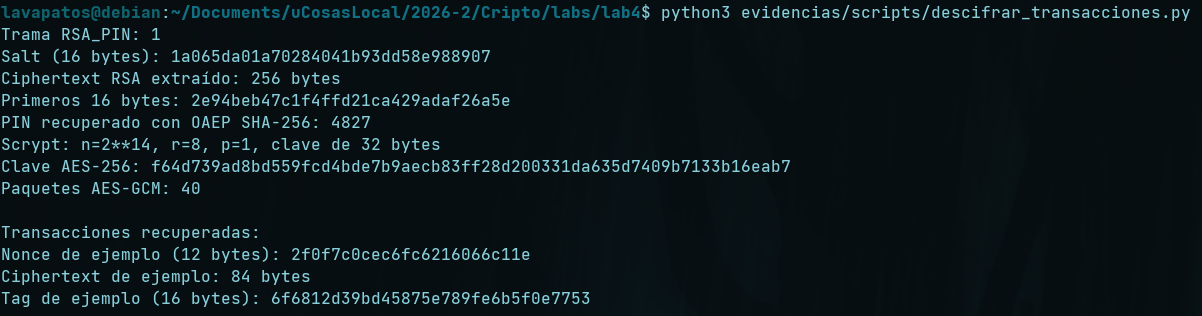
\includegraphics[width=0.98\linewidth]{../evidencias/capturas_informe/14_python_rsa_scrypt_aesgcm.png}
        \caption{Recuperación del PIN y derivación de la clave AES-256 mediante Scrypt.}
        \label{fig:rsa-scrypt}
    \end{figure}

    \subsubsection{Descifrar los mensajes}

    Para cada payload con la etiqueta \texttt{AESGCM|} descarté primero sus 7 bytes.
    Después separé los siguientes 12 bytes como nonce y los últimos 16 como tag; los
    bytes intermedios corresponden al ciphertext. En la trama 2 obtuve el nonce
    \texttt{2f0f7c0cec6fc6216066c11e}, 84 bytes de ciphertext y el tag
    \texttt{6f6812d39bd45875e789fe6b5f0e7753}.

    Usé la clave AES-256 derivada anteriormente para descifrar cada mensaje. La llamada
    \texttt{AESGCM.decrypt} recibe el ciphertext unido a su tag, por lo que además de
    recuperar el texto comprueba su autenticidad. Si el nonce, la clave, el ciphertext o
    el tag fueran incorrectos, la biblioteca produciría una excepción
    \texttt{InvalidTag}. Los 40 paquetes fueron descifrados sin esa excepción, de modo
    que la verificación terminó en \texttt{40/40}.

    Cada texto recuperado trae los campos \texttt{ID}, \texttt{DE}, \texttt{A} y
    \texttt{MONTO}. El script los presenta como identificador, remitente, destinatario y
    monto, respectivamente. Este fue el código utilizado:

    \lstinputlisting[
        language=Python,
        firstline=1,
        lastline=101,
        caption={Script utilizado para recuperar y presentar las transacciones.},
        label={lst:descifrado}
    ]{../scripts/descifrar_transacciones.py}

    \newpage
    \mbox{}\par
    \begin{figure}[H]
        \centering
        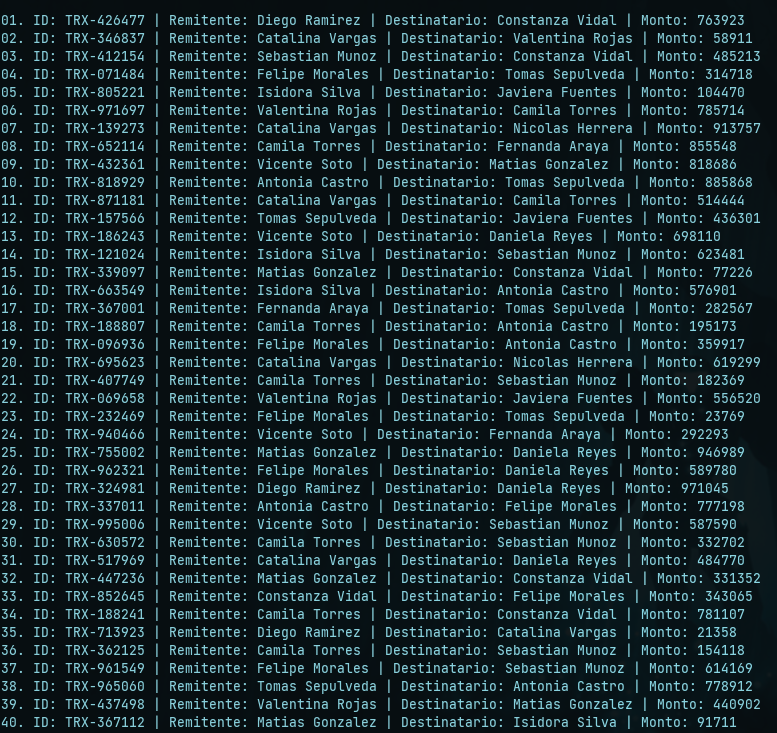
\includegraphics[width=0.95\linewidth]{../evidencias/capturas_informe/15_python_transacciones_y_autenticidad.png}
        \caption{Cuarenta transacciones recuperadas con ID, remitente, destinatario y monto.}
        \label{fig:transacciones}
    \end{figure}

    \newpage
    \mbox{}\par
    \begin{figure}[H]
        \centering
        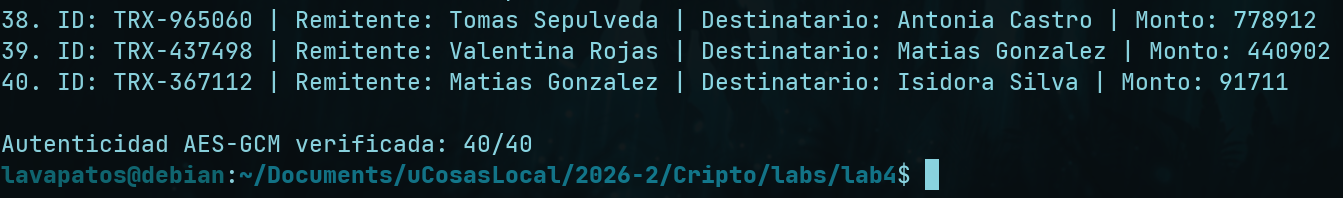
\includegraphics[width=0.98\linewidth]{../evidencias/capturas_informe/16_python_autenticidad_40_de_40.png}
        \caption{Verificación de autenticidad AES-GCM completada para los 40 mensajes.}
        \label{fig:aesgcm-autenticidad}
    \end{figure}

    \subsubsection{RSA frente a criptografía post-cuántica}

    Mi conclusión es que las claves RSA entregadas no permitirían descifrar mensajes
    protegidos exclusivamente mediante un algoritmo post-cuántico como ML-KEM. En este
    laboratorio la clave privada pudo recuperar el PIN porque el ciphertext había sido
    generado con la clave pública RSA correspondiente y se usó OAEP con SHA-256. Es
    decir, tanto el formato de la clave como el del ciphertext pertenecían a RSA.

    ML-KEM no es RSA con otro relleno. Este mecanismo genera una clave de encapsulación
    y otra de decapsulación propias. Para recuperar el secreto compartido se necesita la
    clave de decapsulación ML-KEM que corresponde a ese ciphertext. Una clave privada
    RSA no tiene el formato ni la estructura interna requerida por ML-KEM, por lo que no
    puede reemplazarla.

    El algoritmo de Shor explica por qué RSA sería vulnerable frente a un computador
    cuántico suficientemente potente. Sin embargo, romper RSA no convierte una clave RSA
    en una clave post-cuántica ni permite usarla para decapsular ML-KEM.

    El único caso que requiere un matiz es un esquema híbrido. Si un protocolo combinara
    RSA y ML-KEM, conocer la clave RSA podría comprometer el componente RSA, pero no
    entregaría automáticamente el secreto del componente post-cuántico. En una
    construcción bien diseñada, la clave final depende de ambos resultados, de modo que
    romper solamente RSA no debería bastar mientras ML-KEM continúe siendo seguro. El
    resultado exacto dependería del método usado por el protocolo para combinar ambos
    secretos.

\section*{Conclusiones y comentarios}
\addcontentsline{toc}{section}{Conclusiones y comentarios}

El servidor SSH quedó funcionando dentro del contenedor y accesible solamente desde
\texttt{127.0.0.1:22222}. La configuración efectiva confirmó
\texttt{curve25519-sha256}, \texttt{aes256-ctr}, \texttt{hmac-sha2-256} y
\texttt{ssh-ed25519}. Al principio Wireshark mostraba el tráfico del puerto 22222 solamente
como TCP y fue necesario usar \textit{Decode As} para interpretarlo como SSH. Esta fue la
parte que más me costó entender. Una vez configurado pude observar las direcciones, los
puertos, las versiones de OpenSSH y los algoritmos negociados. Aunque SSH cifra los comandos
y sus respuestas, esa información todavía queda visible en la captura.

En la captura entregada identifiqué una trama \texttt{RSA\_PIN|} y 40 tramas
\texttt{AESGCM|}. Del primer payload extraje la salt de 16 bytes y el ciphertext RSA de
256 bytes. El descifrado OAEP con SHA-256 recuperó el PIN \texttt{4827}; después, Scrypt
con $n=2^{14}$, $r=8$ y $p=1$ produjo la clave AES-256. Con esa clave separé el nonce, el
ciphertext y el tag de cada mensaje. Esto formó una cadena en la que cada resultado era
necesario para el paso siguiente: RSA permitió recuperar el PIN, Scrypt derivó la clave y
AES-GCM descifró las transacciones. La verificación \texttt{40/40} no solo indica que los
mensajes pudieron leerse, sino también que sus tags fueron válidos en los 40 casos.

También quedó claro que una clave privada no sirve para cualquier esquema de cifrado. La
clave RSA entregada permite descifrar el ciphertext RSA correspondiente, pero no puede
reemplazar una clave de decapsulación ML-KEM. Incluso en un sistema híbrido, comprometer RSA
no debería bastar por sí solo si el componente post-cuántico y el método de combinación
siguen siendo seguros.

En general, la actividad se sintió muy guiada. Docker permitió aislar el servidor y probar
la configuración sin modificar directamente el equipo anfitrión, pero no lo consideré
esencial para el objetivo porque SSH también podía configurarse de forma directa. Para mí
fue una herramienta más dentro del procedimiento. También habría preferido una estructura
menos rígida para el informe y mayor libertad para ajustar la geometría de la plantilla, ya
que con las capturas de pantalla fue difícil evitar imágenes demasiado grandes o espacios
mal aprovechados.

\section{Bibliografia}
\thispagestyle{plain}
\begin{itemize}
    \item \href{https://drive.google.com/drive/folders/1rXMp5y9WeBR36iytc4RBaqXKWf3ea-WU} {Captura y Claves}
    \item \href{https://github.com/lavapatos/cripto-labs/tree/main/lab-4}
    {Repositorio del Laboratorio 4 en GitHub}.
    \item IETF, \href{https://www.rfc-editor.org/rfc/rfc8731.html#section-3}
    {RFC 8731: intercambio de claves Curve25519 en SSH, sección 3}.
    \item IETF, \href{https://www.rfc-editor.org/rfc/rfc4344.html#section-4}
    {RFC 4344: modos AES-CTR para SSH, sección 4}.
    \item IETF, \href{https://www.rfc-editor.org/rfc/rfc6668.html#section-2}
    {RFC 6668: HMAC-SHA2 para SSH, sección 2}.
    \item IETF, \href{https://www.rfc-editor.org/rfc/rfc8709.html}
    {RFC 8709: Ed25519 para SSH}.
    \item IETF, \href{https://www.rfc-editor.org/rfc/rfc4253.html#section-6.4}
    {RFC 4253: integridad de paquetes en el protocolo de transporte SSH, sección 6.4}.
    \item IETF, \href{https://www.rfc-editor.org/rfc/rfc8017.html#section-7.1}
    {RFC 8017: RSAES-OAEP, sección 7.1}.
    \item NIST, \href{https://nvlpubs.nist.gov/nistpubs/fips/nist.fips.203.pdf}
    {FIPS 203: estándar ML-KEM}.
    \item NIST, \href{https://nvlpubs.nist.gov/nistpubs/SpecialPublications/NIST.SP.800-227.pdf}
    {SP 800-227: mecanismos de encapsulación y esquemas híbridos}.
    \item NIST, \href{https://nvlpubs.nist.gov/nistpubs/ir/2026/NIST.IR.8547.pdf}
    {IR 8547: transición hacia criptografía post-cuántica}.
\end{itemize}

\end{document}
